\section{总体架构}

系统由医院终端、本地浏览器工作线程、跨域传输通道、业务侧前置网关、服务端权威快检层和两方安全执行域共同组成。明文图像仅在浏览器工作线程中完成解码、裁剪、归一化、数据质量评估与分片生成，跨越信任边界后仅传输密态分片（share）、结构化元数据和审计摘要；服务端在进入 SPU 计算前完成协议与张量合法性检查，随后由两方安全执行链路联合输出最终分类结果。

图 2-1 采用按信任边界分区的部署拓扑：左侧为医院终端与本地明文处理域，中间为广域网与隔离缓冲区（wide area network / demilitarized zone, WAN/DMZ）传输边界，右侧为业务侧前置网关、服务端权威快检层与参与方安全执行域。图中显式标注了明文终止点和密态分片生成起点，并以差异化图例区分本地明文处理与跨边界密态通信。

\begin{figure}[htbp]
\centering
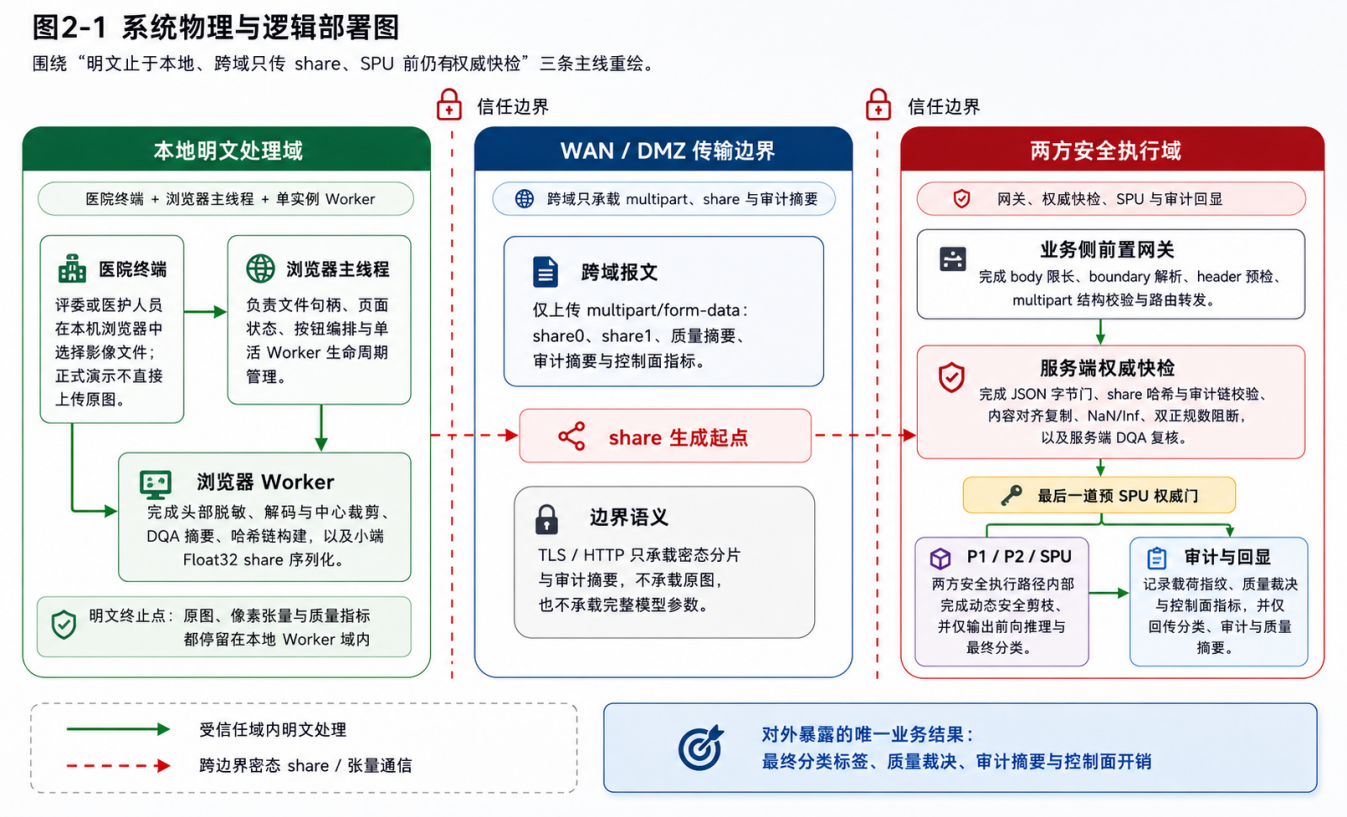
\includegraphics[width=0.92\textwidth]{figures/fig2-1-system-topology.png}
\caption{图2-1 系统物理与逻辑部署图：绿色实线表示本地明文处理，红色虚线与锁图标表示跨越信任边界的密态分片与张量通信。}
\end{figure}

\section{软件流程}

图 2-2 给出了完整的软件流转时序。主线程仅负责本地影像加载、预览和请求编排；浏览器工作线程独立完成图像解码、裁剪、数据质量评估指标提取、审计链构建与分片序列化；服务端首先执行原始报文体、边界参数、报文头与多部件结构校验，再对结构化元数据、密态分片与重构张量进行权威快检，全部通过后方可进入 SPU 密态前向计算。最终结果回传时同时包含分类结论、质量裁决、审计摘要与控制面开销，使展示链路与安全链路保持一致。

\begin{figure}[htbp]
\centering
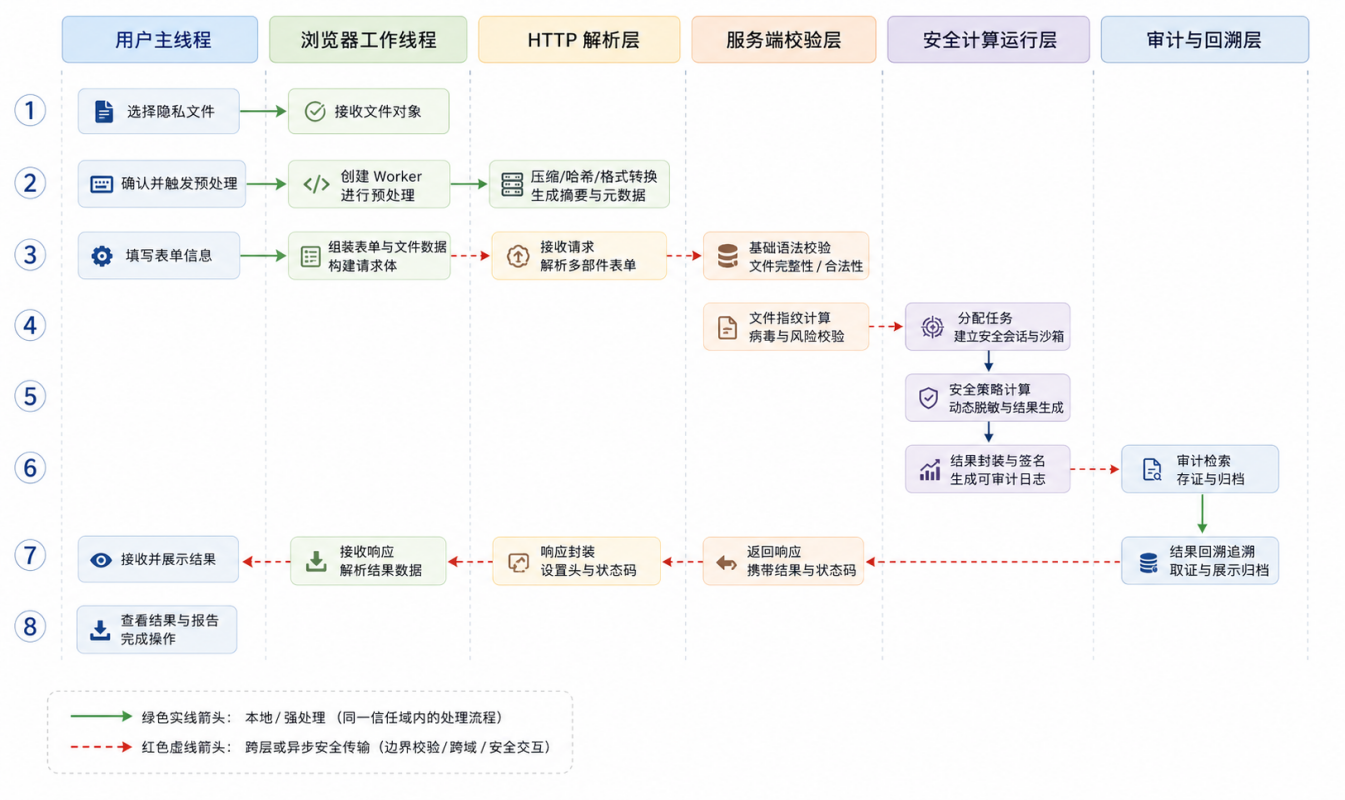
\includegraphics[width=0.92\textwidth]{figures/fig2-2-software-sequence.png}
\caption{图2-2 端到端软件流转时序图：明文仅停留在浏览器工作线程域内，跨域仅传输密态分片与审计摘要。}
\end{figure}

\section{威胁模型与安全边界}

本作品采用两方半诚实威胁模型。系统中，医院终端持有原始输入数据，模型持有方与协同计算方分别持有安全执行域中的不同份额。参与方均遵循协议执行，但可能试图从交互过程中推断对方的隐私信息。系统假设两方不串谋，且不考虑恶意篡改协议、主动注入畸形中间值或侧信道攻击等更强对抗情形。

本作品保护的对象包括：原始影像、模型参数、中间特征、动态剪枝路径以及最终推理结果；系统允许暴露的对象仅包括最小必要的结构化元数据、审计摘要和最终分类结论。本文不声称覆盖生产环境中所有攻击面，尤其不覆盖恶意共谋、模型抽取、物理侧信道和输出反推风险。系统的威胁模型、保护对象与安全边界核心定义如表 1 所示。

\begin{longtable}{>{\raggedright\arraybackslash}p{0.48\textwidth}>{\raggedright\arraybackslash}p{0.48\textwidth}}
\caption{表 1 系统威胁模型与安全边界定义}\\
\toprule
\textbf{项目} & \textbf{说明} \\
\midrule
\endfirsthead
\toprule
\textbf{项目} & \textbf{说明} \\
\midrule
\endhead
保护对象 & 用户输入数据、模型参数、中间动态决策状态、审计与控制面证据 \\
参与方 & 医院终端浏览器、浏览器工作线程、业务侧前置网关、服务端快检模块、两方 SPU 节点 \\
攻击者能力 & 可监听网络、构造畸形多部件表单报文（multipart/form-data）、伪造结构化元数据、重放一次性随机标识（nonce）、提交异常密态分片、实施并发探测 \\
安全假设 & 两方半诚实；不引入额外可信第三方；前端不作为可信根，关键裁决以服务端复算为准 \\
不覆盖范围 & 恶意参与方串谋、浏览器被完全控制、进入长耗时 SPU 后的主动断连感知、生产级分布式 DoS、防输出反演攻击 \\
防护证据 & 协议层模糊测试、重放与并发守卫测试、服务端张量快检与审计落盘证据 \\
\bottomrule
\end{longtable}

\noindent\textit{注：本表格基于两方半诚实威胁模型制定，仅覆盖原型系统设计范围内的安全假设与防护边界，不代表生产级系统的完整安全承诺}

\begin{longtable}{>{\raggedright\arraybackslash}p{0.32\textwidth}>{\raggedright\arraybackslash}p{0.32\textwidth}>{\raggedright\arraybackslash}p{0.32\textwidth}}
\caption{表 2 系统各维度安全边界覆盖情况}\\
\toprule
\textbf{边界项} & \textbf{当前覆盖} & \textbf{当前不覆盖或限制} \\
\midrule
\endfirsthead
\toprule
\textbf{边界项} & \textbf{当前覆盖} & \textbf{当前不覆盖或限制} \\
\midrule
\endhead
输入明文保护 & 明文图像只在浏览器工作线程内解码、裁剪与分片，服务端仅接收密态 share 与结构化元数据 & 不覆盖浏览器被完全控制或本地终端失陷后的明文窃取 \\
模型参数保护 & 模型参数不向数据使用方以明文暴露，仅在两方安全执行域内参与计算 & 不覆盖恶意参与方串谋、模型抽取与生产级侧信道分析 \\
动态决策隐私 & PredictorLG、阈值判断与并列分数决断保留在安全执行域内 & 不覆盖进入安全图后的主动任务取消、长连接断开感知与更强攻击模型 \\
协议与输入防护 & 原始多部件表单预检、JSON（JavaScript Object Notation）字节门、share 哈希与张量合法性快检、重放与并发守卫已落地 & 不覆盖生产级分布式 DoS、跨节点全局限流与外部 WAF/网关联动 \\
审计与复现 & nonce、请求载荷（payload）、质量摘要与审计事件落盘，报告与脚本可回溯 & 不覆盖长期合规归档平台、外部 SIEM 集成与跨系统追责链 \\
\bottomrule
\end{longtable}

\noindent\textit{注："当前覆盖" 项均已通过黑盒验证并留存审计证据；"当前不覆盖或限制" 项为原型系统明确不承诺的防护能力，需在生产部署中补充对应机制。}

各维度安全边界的具体覆盖情况与明确未覆盖范围如表 2所示，上述边界说明用于避免将原型级控制面夸大为生产级防御体系。更完整的未覆盖范围、输出侧风险与原型部署边界，统一放在第 5.5 节“当前局限性”中说明。

为便于从步骤层面概括端到端链路，算法1给出本作品从终端预处理、秘密分享、服务端预检到密态推理与结果回传的完整流程。该流程与图2-2所示时序一致，强调了明文仅停留在终端侧、跨域仅传输密态分片与审计摘要的边界约束。

从部署视角看，威胁模型不仅决定密码学协议选择，也决定系统哪些组件能够接触明文、哪些组件只能处理密态分片。许多系统只在算法层声明“保护输入与模型”，但不进一步说明原始文件、预处理张量、结构化元数据和审计记录分别落在何处。本作品在威胁模型中显式规定：原始影像与明文像素止于终端侧，跨边界传输对象被限制为 share、结构化元数据和审计摘要，服务端仅在全部快检通过后触发安全执行。这种“边界先于协议”的约束，是后续控制面设计和部署骨架成立的前提。

在安全边界之外，系统还需要处理“元数据最小化”问题。实际部署时，完全隐藏所有运行状态并不现实，因为服务端需要依据尺寸、哈希、质量摘要和任务标识完成预检、去重、审计与资源调度；但如果元数据过多，又可能间接泄露输入分布或动态路径。本作品采用最小必要原则，只保留验证任务完整性和运行可追溯所需的结构化字段，并将原始像素、明文张量、模型权重和剪枝决策限制在相应安全边界内。该设计为后续从本机展示样例迁移到医院侧与模型提供方分离部署提供了统一约束。

\section{DynamicViT 密态改写}

原始 DynamicViT 中四类核心操作的安全计算困难点、本作品的改写方案、代价与验证方式如表 3 所示。

\begin{longtable}{>{\raggedright\arraybackslash}p{0.19\textwidth}>{\raggedright\arraybackslash}p{0.19\textwidth}>{\raggedright\arraybackslash}p{0.19\textwidth}>{\raggedright\arraybackslash}p{0.19\textwidth}>{\raggedright\arraybackslash}p{0.19\textwidth}}
\caption{表 3 DynamicViT 原始操作与密态语义改写对照表}\\
\toprule
\textbf{原始DynamicViT操作} & \textbf{安全计算困难} & \textbf{本作品改写方式} & \textbf{代价} & \textbf{验证方式} \\
\midrule
\endfirsthead
\toprule
\textbf{原始DynamicViT操作} & \textbf{安全计算困难} & \textbf{本作品改写方式} & \textbf{代价} & \textbf{验证方式} \\
\midrule
\endhead
直接删除 token & 变长结构难以进入固定图安全执行，且会暴露路径 & 改写为保留/置零的掩码化表达（keep/zero），由安全选择完成保留决策 & 保留了部分冗余计算 & 本地明文参考路径与 secure replay 一致性对齐 \\
明文阈值比较 & 数据相关分支会泄露剪枝边界 & 将比较逻辑改写为安全比较语义 & 增加比较通信与控制流复杂度 & 部署阈值回代与输出一致性验证 \\
数据相关 Top-选择 & 动态索引与并列分数处理不稳定 & 采用编码索引跟踪与排序网络构造保留掩码（keep-mask） & 排序代价上升 & 排序结果与后续决策链功能验证 \\
外部明文决定 keep-mask & 会退化为半隐私运行 & 将 PredictorLG、阈值判断和并列分数决断（tie）保留在安全执行域内 & 图规模扩大、执行时间增长 & 双向隐私运行链与前端控制面联调 \\
\bottomrule
\end{longtable}

\noindent\textit{注：所有改写操作均在 SecretFlow SPU 0.9.3.dev20241118 框架下实现，验证方式包含本地明文参考对齐与密态执行一致性校验。}

为便于从工程层面理解本节中的协议友好重写，图 2-3 将原始 DynamicViT 的删除式剪枝路径与本作品的掩码化密态语义重写并列展示。其核心差异在于：正式交付链路不再直接删除词元，而是以 keep-mask 表达保留边界，从而在固定图安全执行约束下保留动态剪枝能力。

\begin{figure}[htbp]
\centering
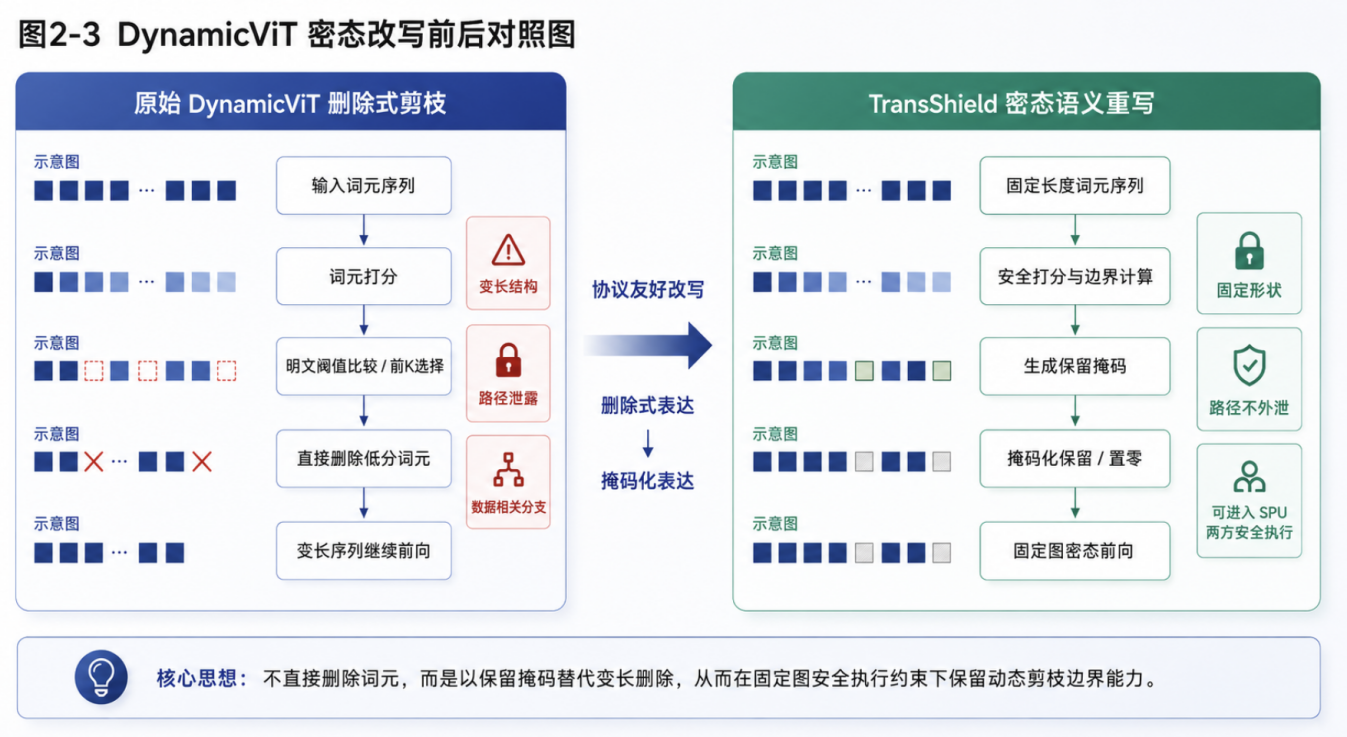
\includegraphics[width=0.92\textwidth]{figures/fig2-3-pruning-rewrite.png}
\caption{图2-3 DynamicViT 密态改写前后对照图：左侧为原始删除式剪枝，右侧为本作品的掩码化重写与固定图密态前向。}
\end{figure}

\section{硬件部署与软件基准}

本作品所有实验与性能测试均在统一的硬件与软件环境下执行，具体配置基准如表 4 所示。

\begin{longtable}{>{\raggedright\arraybackslash}p{0.48\textwidth}>{\raggedright\arraybackslash}p{0.48\textwidth}}
\caption{表 4 原型系统硬件部署与软件环境基准}\\
\toprule
\textbf{项目} & \textbf{配置} \\
\midrule
\endfirsthead
\toprule
\textbf{项目} & \textbf{配置} \\
\midrule
\endhead
CPU & Intel Xeon Gold 6148 @ 2.40GHz，80 逻辑核（2 路，每路 20 核，超线程开启） \\
物理内存 & 62 GiB \\
操作系统 & Ubuntu 20.04.6 LTS \\
内核版本 & Linux 5.15.0-139-generic \\
Python & Python 3.9.25 \\
安全计算底座 & SecretFlow SPU 0.9.3.dev20241118（Apache License 2.0） \\
原型运行模式 & 两方 2PC colocated localhost 原型链路，通信量来自同配置 fresh rerun 的 SPU LinkDetails 计数器 \\
GPU & 服务器侧配备 4 张 NVIDIA GeForce RTX 3090 GPU，单卡显存 24576 MiB（约 24 GiB），驱动版本为 570.133.07，CUDA 版本为 12.8。 \\
\bottomrule
\end{longtable}

需要说明的是，表 4 记录的是当前原型系统在统一软件栈和统一硬件条件下的实验基准，而不是医院生产环境的最终配置。安全推理时延同时受到协议轮次、矩阵规模、底层数值库、并发方式和网络条件影响；若脱离统一环境去比较动态主线、静态基线与外部相关工作，结论容易失真。因此，后续章节中出现的通信量、端到端时延和鲁棒性指标，均默认建立在本节给出的统一基准之上。

\section{展示样例与真实部署框架}

为区分原型演示与后续部署边界，本作品在工程实现中将系统形态划分为“本机展示样例”和“真实部署框架”两类。本机展示样例用于验证端到端流程：系统在一台机器上启动本地双节点安全处理器单元（Secure Processing Unit, SPU），由展示站前端完成图像选择、预处理与分片生成，后端完成协议校验、审计记录和密态前向计算，形成可运行、可追踪的闭环。

真实部署框架面向医院侧与模型提供方分离部署。该框架保留了 public manifest、P1/P2 party manifest、单方 share 加载、远程 2PC 配置生成、医院侧/AI 侧/协调侧三类网关角色以及部署包生成脚本。医院侧负责原始影像接收、预处理与 P1 share 留存，AI 或模型提供方负责 P2 share 与模型 manifest 管理，协调侧负责公开任务状态、运行编排和最终可公开结果的返回。

二者对应同一安全推理思想下的不同交付层次：本机展示样例证明流程可运行、可审计、可复现；真实部署框架提供向两方部署迁移的接口、配置和脚本骨架。当前框架提供的是部署迁移基础，不直接覆盖生产环境中的医院 HIS/PACS 接入、机构身份认证、TLS/VPN、长期审计、任务队列、密钥管理和模型私有加载策略，相关内容需要在具体医院与模型提供方环境中按现场规范继续集成。
